\chapter{Test Journal: DC motor velocity constant $\boldsymbol{K_e}$} \label{test:Ke}
\begin{table}[!h]
\begin{tabular}{l l}
\textbf{Test participants:} & Maxime, Robin \& Bang  \\
\textbf{Date:}  & 14/10-2016
\end{tabular}
\end{table}

\section*{Purpose}
The purpose of the test is to determine the velocity constant $K_e$ of the DC motor. 
\section*{Test equipment and components}
The test equipment and components are listed in \autoref{tab_appendix:testKe1}.
\begin{table}[h]
	\centering
	\caption{List of measurement equipment and components}\label{tab_appendix:testKe1}

	\begin{tabularx}{\textwidth}{lXXXX}
		Name 				& Brand	& Model & AAU-number									\\ \toprule \rowcolor{lightGrey}
		Two multimeters	& Fluke & 37 & 08181 \& 33045	\\
		Powersupply	& Hameg triple & HM7042 & 33902\\ \rowcolor{lightGrey}
		DC motor & Maxon & 41.023.038-00.00-052& N/A \\
		Tachometer, laser & Compact instruments & A2103/LSR & N/A \\ \rowcolor{lightGrey}
		\SI{30.2}{\ohm} resistor & N/A & N/A & N/A \\ 
	\end{tabularx}
\end{table}
\section*{Setup}
Diagram of the setup is illustrated on \autoref{fig:KE:DCR_circuit} and a picture of the measurement setup is given on \autoref{fig:KE:DCR_setup}. 
\begin{figure}[h!]
    \centering
    \begin{subfigure}{0.50\textwidth}
        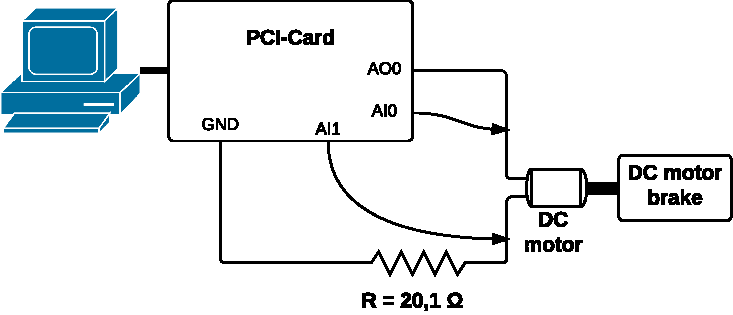
\includegraphics[width=1\textwidth]{figures/design/DCR_circuit}
        \caption{Diagram of the setup.} \label{fig:KE:DCR_circuit}
    \end{subfigure}
    \begin{subfigure}{0.40\textwidth}
        \includegraphics[width=1\textwidth]{figures/design/ke_meas}
        \caption{Picture of the setup.} \label{fig:KE:DCR_setup}
    \end{subfigure}
    \caption{The measurement setup.}    
\end{figure}

\section*{Method}
The DC motor with a known resistor in series, is set up as seen on \autoref{fig:KE:DCR_circuit}. Two multimeters are connected to the circuit, to measure voltage, one across the resistor and one across the DC motor. The tachometer measures the rotational speed of the motor shaft.% in \gls{rpm} (It do not have to be messured in \gls{rpm}, but for this test it was). 
\begin{enumerate}
\item Set the supply voltage at a certain voltage.
\item Wait for DC motor to reach steady state.
\item Read the voltage across the resistor and DC motor.
\item Read the rotational speed of the motors rotational body.
\item Repeat steps 1 to 4 with different supply voltages.
\end{enumerate}
\section*{Results}
The results from the test are listed in \autoref{tab_appendix:testKe2}.
\begin{table} [!h]
	\centering
	\caption{Data of the measurement}\label{tab_appendix:testKe2}
	\begin{tabularx}{\textwidth}{llX}
		Voltage over the resistor [\si{\volt}]& Voltage over the DC Motor [\si{\volt}]	& 	\gls{rpm} [\si{\per\minute}]						\\ \toprule \rowcolor{lightGrey}
0.17 & 1.05 & 14.30	\\
0.22 & 1.05 & 29.30 \\ \rowcolor{lightGrey}
0.28 & 3.00 & 44.50 \\
0.33 & 4.04 & 60.80 \\ \rowcolor{lightGrey}
0.38 & 5.20 & 79.00 \\
0.45 & 6.55 & 100.40 \\ 
	\end{tabularx}
\end{table}

\newpage
\section*{Data processing}
With the known resistor and the voltage across it, the current through the circuit can be calculated with Ohms law.
The speed of the DC motor it is calculated from \gls{rpm} to angular velocity with \autoref{appendix:eq:KeRPMtoRads}
\begin{equation}
\omega_m = \frac{RPM \cdot 2 \pi}{60}\addunit{\si{\radian\per\second}} \label{appendix:eq:KeRPMtoRads}
\end{equation}

By analysing the electric model of the DC motor, shown on \autoref{fig:DC_diagram}, kirchhoffs voltage law can be used to set up an equation for the velocity constant $K_e$.
\begin{figure} [h!]
\centering
\includegraphics[width=0.6\linewidth]{figures/design/electrical_model_motor}
\caption{Diagram of the electric model of a DC motor \citep{ModelingAndAnalisys}.}
\label{fig:DC_diagram}
\end{figure} 

When the DC motor reaches steady state, the voltage drop across the inductor is 0. Kirchhoffs equation is then given as \autoref{appendix:eq:BmKirchhoff}.
\begin{equation}
V_s= R_a  i_a + K_e  \omega_m \implies K_e = \frac{V_s - R_a i_a}{\omega_m} \addunit{\si{\volt\second\per\radian}} \label{appendix:eq:BmKirchhoff}
\end{equation}
Result from the calculations can be seen on \autoref{tab_appendix:testKe3}.

\begin{table}[!h]
	\centering
	\caption{Data of the measurement}\label{tab_appendix:testKe3}
	\begin{tabularx}{\textwidth}{XXX}
		$i_a$ [$\SI{}{mA}$]& $\omega_m$ [$\SI{}{\radian\per\second}$]	& $K_e$ [$\SI{}{\volt\second\per\radian}$]									\\ \toprule \rowcolor{lightGrey}
		5.53 & 1.50 & 0.579	\\
		7.38 & 3.07 & 0.576 \\ \rowcolor{lightGrey}
		9.27 & 4.66 & 0.578 \\
		10.93 & 6.37 & 0.577 \\ \rowcolor{lightGrey}
		12.68 & 8.27 & 0.577 \\
		14.90 & 10.51 & 0.576 \\ 
	\end{tabularx}
\end{table}

\newpage
\section*{Conclusion}
The test show that the velocity constant is $K_e\approx\SI{0.577}{\volt\second\per\radian}$.